% !TEX spellcheck = en_US



% ~~~~~~~~~~~~~~~~~~~~~~~~~~~~~~~~~~~~~~~ V
% (NC) 2026 Haluk Bingol
% github.com/halukbingol/LaTeX-Templates
%
% Licensees may copy, distribute, display, and perform the work and make derivative works 
% and remixes based on it only for non-commercial purposes. 
% ~~~~~~~~~~~~~~~~~~~~~~~~~~~~~~~~~~~~~~~ A




% =====================================================================
%  Maven for Java -- Senior Level: The Model, Dependency Resolution, Reproducibility, Plugins and Publishing
%  ---------------------------------------------------------------------
%  Built on hblib/Template/hblibTemplate.tex with the libraries in ../../hblib/.
%  Programs and their real outputs are in codeoutput/:
%     codeoutput/<Name>.java  a program (classes without main() are only compiled)
%     codeoutput/<Name>.sh    a terminal session, run in a copy of codeoutput/<Name>/
%     codeoutput/<Name>.txt   what it printed, made by:  bash run_examples.sh
% =====================================================================

\documentclass[aspectratio=169,10pt,compress]{beamer}

% ~~~~~~~~~~~~~~~~~~~~~~~~~~~~~~~~~~~~~~~~~~~~~~~~~~~~~~~~~~~~~~~~~ V hblib
	\usepackage{../../hblib/hblibPresentation} % lib presentation: theme, i/N, \hSection, algorithm2e, ...
	\usepackage{../../hblib/hblibCodeoutput} % lib code + output: \lstcode, \lstterminal, ...
	\usepackage{../../hblib/hblibDatastructures} % lib data structures: \hString, \hStack, \hQueue
% ~~~~~~~~~~~~~~~~~~~~~~~~~~~~~~~~~~~~~~~~~~~~~~~~~~~~~~~~~~~~~~~~~ A hblib


% theme, i/N, fonts (T1, lmodern), booktabs, xcolor, array (L{width} columns), listings, tikz,
% algorithm2e (\small captions, \Fn) and the color gitred come from the hblib libraries




% +++++++++++++++++++++++++++++++++++++++ V specific
\DontPrintSemicolon % in algorithms
\newcommand{\win}{\textbf{Windows}}
\newcommand{\mac}{\textbf{macOS}}
% +++++++++++++++++++++++++++++++++++++++ A specific

% ---------------------------------------------------------------------
\title{Maven for Java}
\subtitle{Senior Level: The Model, Dependency Resolution, Reproducibility, Plugins and Publishing}
\author[Bingol]{Haluk O. Bingol}

\institute[FCIS]{
    Faculty of Computer and Information Sciences\\
    Yeditepe University
}
\date{
	{\tiny \hbTimeStamp}
}

\begin{document}




% ~~~~~~~~~~~~~~~~~~~~~~~~~~~~~~~~~~~~~~ V frm
\begin{frame}[t,fragile]
  \titlepage
\end{frame}
% ~~~~~~~~~~~~~~~~~~~~~~~~~~~~~~~~~~~~~~ A frm




% ~~~~~~~~~~~~~~~~~~~~~~~~~~~~~~~~~~~~~~ V frm
\begin{frame}[t,fragile] \frametitle{Outline}
  \begin{columns}[T]
    \begin{column}{0.48\textwidth}
      \tableofcontents[sections={1-5}, hideallsubsections]
    \end{column}
    \begin{column}{0.48\textwidth}
      \tableofcontents[sections={6-10}, hideallsubsections]
    \end{column}
  \end{columns}
\end{frame}
% ~~~~~~~~~~~~~~~~~~~~~~~~~~~~~~~~~~~~~~ A frm

% ~~~~~~~~~~~~~~~~~~~~~~~~~~~~~~~~~~~~~~ V
\hSection[Model]{The Project Model}
% ~~~~~~~~~~~~~~~~~~~~~~~~~~~~~~~~~~~~~~ A




% ~~~~~~~~~~~~~~~~~~~~~~~~~~~~~~~~~~~~~~ V frm
\begin{frame}[t,fragile] \frametitle{Where a setting comes from}
  \begin{columns}[T]
    \begin{column}{0.44\textwidth}
      \begin{center}
      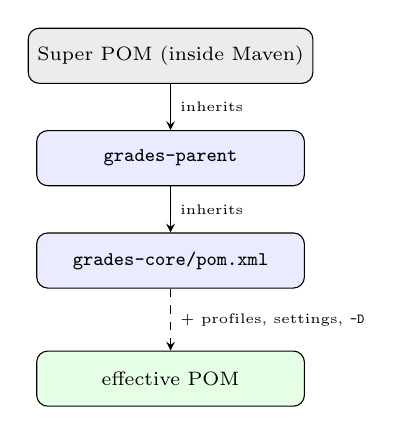
\begin{tikzpicture}[box/.style={draw, rounded corners, fill=blue!8, font=\scriptsize, minimum width=3.4cm, minimum height=0.7cm, align=center}, >=stealth]
        \node[box, fill=gray!15] (s) at (0,0)    {Super POM (inside Maven)};
        \node[box]               (p) at (0,-1.3) {\texttt{grades-parent}};
        \node[box]               (c) at (0,-2.6) {\texttt{grades-core/pom.xml}};
        \node[box, fill=green!10] (e) at (0,-4.1) {effective POM};
        \draw[->] (s) -- node[right, font=\tiny] {inherits} (p);
        \draw[->] (p) -- node[right, font=\tiny] {inherits} (c);
        \draw[->, dashed] (c) -- node[right, font=\tiny] {+ profiles, settings, \texttt{-D}} (e);
      \end{tikzpicture}
      \end{center}
    \end{column}
    \begin{column}{0.54\textwidth}
      \begin{itemize}\small
        \item The \textbf{Super POM} gives the conventions: \texttt{src/main/java}, \texttt{target}, Maven Central.
        \item Each POM \emph{merges} into its parent's: single values are replaced, lists (dependencies, plugins) merged by key.
        \item Then active profiles, then \texttt{\$\{\dots\}} interpolation (\texttt{project.*}, \texttt{env.*}, properties, \texttt{-D}).
        \item The result, the \textbf{effective POM}, is what Maven really builds: \texttt{mvn help:effective-pom} (help plugin, not run here).
        \item Inheritance (\texttt{<parent>}) and aggregation (\texttt{<modules>}) are independent: one can have either without the other.
      \end{itemize}
    \end{column}
  \end{columns}
\end{frame}
% ~~~~~~~~~~~~~~~~~~~~~~~~~~~~~~~~~~~~~~ A frm

% ~~~~~~~~~~~~~~~~~~~~~~~~~~~~~~~~~~~~~~ V
\hSection[Resolution]{Dependency Resolution}
% ~~~~~~~~~~~~~~~~~~~~~~~~~~~~~~~~~~~~~~ A




% ~~~~~~~~~~~~~~~~~~~~~~~~~~~~~~~~~~~~~~ V frm
\begin{frame}[t,fragile] \frametitle{Mediation: one version per artifact}
  \begin{columns}[T]
    \begin{column}{0.58\textwidth}


% +++++++++++++++++++++++++++++++++++++++ V alg
%: -Alg. 
\begin{algorithm}[H]
  \caption{Dependency mediation (Maven 3)}
  \KwIn{direct dependencies $d_{1}, \dots, d_{n}$, in declared order}
  queue $Q \leftarrow (d_{1}, 1), \dots, (d_{n}, 1)$; \ $C \leftarrow \emptyset$\;
  \While{$Q$ is not empty}{
    $(d, k) \leftarrow$ dequeue $Q$\;
    \lIf{$d$ is managed}{$d.\mathit{version} \leftarrow$ the managed version}
    \lIf{$C$ has $d.\mathit{ga}$}{\textbf{continue}\tcp*[h]{omitted for conflict}}
    $C[d.\mathit{ga}] \leftarrow d$\;
    \lForEach{dependency $e$ of $d$ (scope, optional, exclusions)}{enqueue $(e, k+1)$}
  }
  \Return{$C$}
\end{algorithm}
% +++++++++++++++++++++++++++++++++++++++ A alg

    \end{column}
    \begin{column}{0.4\textwidth}
      \begin{itemize}\small
        \item Breadth first: the \textbf{nearest} declaration wins; at equal depth, the \textbf{first} declared.
        \item Not the newest! Maven does not compare versions here.
        \item \texttt{dependencyManagement} overrides any depth; optional dependencies and exclusions cut branches.
      \end{itemize}
    \end{column}
  \end{columns}
\end{frame}
% ~~~~~~~~~~~~~~~~~~~~~~~~~~~~~~~~~~~~~~ A frm




% ~~~~~~~~~~~~~~~~~~~~~~~~~~~~~~~~~~~~~~ V frm
\begin{frame}[t,fragile] \frametitle{Nearest wins, even if older}
  \lstterminal[basicstyle=\ttfamily\tiny]{codeoutput/Nearest.txt}

  \vspace{0.1em}
  \small
  \texttt{textutil} 1.0 is declared directly (depth 1); \texttt{lib-b} needs 2.0 (depth 2). Depth 1 wins: \texttt{NoSuchMethodError} at run time. Your direct dependency is a promise that it fits all users.
\end{frame}
% ~~~~~~~~~~~~~~~~~~~~~~~~~~~~~~~~~~~~~~ A frm




% ~~~~~~~~~~~~~~~~~~~~~~~~~~~~~~~~~~~~~~ V frm
\begin{frame}[t,fragile] \frametitle{Scopes along the path}
  \begin{center}\small
  \begin{tabular}{@{}lcccc@{}}
    \toprule
    \textbf{direct $\downarrow$ \ / \ transitive $\rightarrow$} & \texttt{compile} & \texttt{provided} & \texttt{runtime} & \texttt{test} \\
    \midrule
    \texttt{compile}    & compile  & --- & runtime & --- \\
    \texttt{provided}   & provided & --- & provided & --- \\
    \texttt{runtime}    & runtime  & --- & runtime & --- \\
    \texttt{test}       & test     & --- & test    & --- \\
    \bottomrule
  \end{tabular}
  \end{center}
  \begin{itemize}\small
    \item \texttt{provided} and \texttt{test} dependencies of a library never reach its users (---).
    \item A \texttt{compile} dependency of a \texttt{test} dependency becomes \texttt{test}: JUnit's own jars on the previous decks.
    \item \texttt{<optional>true</optional>}: needed to build the library, not passed on (users who need the feature add it).
  \end{itemize}
\end{frame}
% ~~~~~~~~~~~~~~~~~~~~~~~~~~~~~~~~~~~~~~ A frm




% ~~~~~~~~~~~~~~~~~~~~~~~~~~~~~~~~~~~~~~ V frm
\begin{frame}[t,fragile] \frametitle{Version ranges}
  \lstterminal[basicstyle=\ttfamily\tiny]{codeoutput/Range.txt}

  \vspace{0.1em}
  \small
  \texttt{[1.0,3.0)}: any version from 1.0 up to, not including, 3.0; Maven took the highest it knows, 2.0. Ranges make the build depend on the day: prefer fixed versions, pinned in one place.
\end{frame}
% ~~~~~~~~~~~~~~~~~~~~~~~~~~~~~~~~~~~~~~ A frm




% ~~~~~~~~~~~~~~~~~~~~~~~~~~~~~~~~~~~~~~ V frm
\begin{frame}[t,fragile] \frametitle{Releases and snapshots}
  \begin{itemize}\small
    \item A \textbf{release} (\texttt{1.0}) never changes once published; repositories refuse to overwrite it.
    \item A \textbf{snapshot} (\texttt{1.0-SNAPSHOT}) is ``the latest build of 1.0 so far''; deployed copies get time stamps (\texttt{1.0-20261027.090000-3}).
    \item Maven checks remote snapshots once a day by default; \texttt{-U} forces it now, \texttt{-o} (offline) never.
    \item A release must not depend on snapshots: the \texttt{requireReleaseDeps} enforcer rule checks it.
    \item How Maven orders versions: next slide.
  \end{itemize}
\end{frame}
% ~~~~~~~~~~~~~~~~~~~~~~~~~~~~~~~~~~~~~~ A frm




% ~~~~~~~~~~~~~~~~~~~~~~~~~~~~~~~~~~~~~~ V frm
\begin{frame}[t,fragile] \frametitle{How Maven compares versions}
  \lstterminal[basicstyle=\ttfamily\tiny]{codeoutput/Order.txt}

  \vspace{0.1em}
  \small
  \texttt{maven-artifact} (in the \texttt{lib} folder of Maven; Windows: \texttt{\%MAVEN\_HOME\%\textbackslash lib}) compares versions: \texttt{alpha} $<$ \texttt{beta} $<$ \texttt{rc} $<$ \texttt{SNAPSHOT} $<$ release; \texttt{1.10} $>$ \texttt{1.9}.
\end{frame}
% ~~~~~~~~~~~~~~~~~~~~~~~~~~~~~~~~~~~~~~ A frm

% ~~~~~~~~~~~~~~~~~~~~~~~~~~~~~~~~~~~~~~ V
\hSection[BOM]{Bills of Materials}
% ~~~~~~~~~~~~~~~~~~~~~~~~~~~~~~~~~~~~~~ A




% ~~~~~~~~~~~~~~~~~~~~~~~~~~~~~~~~~~~~~~ V frm
\begin{frame}[t,fragile] \frametitle{A BOM: versions that belong together}
  \begin{columns}[T]
    \begin{column}{0.46\textwidth}
      \lstcode[basicstyle=\ttfamily\tiny, firstline=6, firstnumber=6, lastline=29]{codeoutput/Bom/campus-bom/pom.xml}{XML}
    \end{column}
    \begin{column}{0.52\textwidth}
      \lstcode[basicstyle=\ttfamily\tiny, firstline=10, firstnumber=10, lastline=20]{codeoutput/Bom/pom.xml}{XML}
      \lstcode[basicstyle=\ttfamily\tiny, firstline=27, firstnumber=27, lastline=36]{codeoutput/Bom/pom.xml}{XML}
    \end{column}
  \end{columns}
\end{frame}
% ~~~~~~~~~~~~~~~~~~~~~~~~~~~~~~~~~~~~~~ A frm




% ~~~~~~~~~~~~~~~~~~~~~~~~~~~~~~~~~~~~~~ V frm
\begin{frame}[t,fragile] \frametitle{Importing the BOM}
  \lstterminal[basicstyle=\ttfamily\tiny]{codeoutput/Bom.txt}

  \vspace{0.1em}
  \small
  \texttt{scope import} copies the BOM's \texttt{dependencyManagement}: no versions in the project, and \texttt{textutil} 2.0 everywhere. Real BOMs: \texttt{junit-bom}, \texttt{spring-boot-dependencies}, \texttt{jackson-bom}. Unlike a parent, any number of BOMs can be imported.
\end{frame}
% ~~~~~~~~~~~~~~~~~~~~~~~~~~~~~~~~~~~~~~ A frm

% ~~~~~~~~~~~~~~~~~~~~~~~~~~~~~~~~~~~~~~ V
\hSection[Reproducible]{Reproducible Builds}
% ~~~~~~~~~~~~~~~~~~~~~~~~~~~~~~~~~~~~~~ A




% ~~~~~~~~~~~~~~~~~~~~~~~~~~~~~~~~~~~~~~ V frm
\begin{frame}[t,fragile] \frametitle{Same sources, different jars}
  \lstterminal[basicstyle=\ttfamily\scriptsize]{codeoutput/ReproNo.txt}

  \vspace{0.1em}
  \small
  A jar is a zip file with a time stamp for each entry: two builds two seconds apart differ. Nobody can check that a published jar was built from the published sources.
\end{frame}
% ~~~~~~~~~~~~~~~~~~~~~~~~~~~~~~~~~~~~~~ A frm




% ~~~~~~~~~~~~~~~~~~~~~~~~~~~~~~~~~~~~~~ V frm
\begin{frame}[t,fragile] \frametitle{Same sources, same jar}
  \lstterminal[basicstyle=\ttfamily\scriptsize]{codeoutput/ReproYes.txt}

  \vspace{0.1em}
  \small
  \texttt{project.build.outputTimestamp} fixes all time stamps (here \texttt{2026-10-27T09:00:00Z}; shown in local time by \texttt{unzip}). Identical bytes: anyone can rebuild and compare the hash.
\end{frame}
% ~~~~~~~~~~~~~~~~~~~~~~~~~~~~~~~~~~~~~~ A frm

% ~~~~~~~~~~~~~~~~~~~~~~~~~~~~~~~~~~~~~~ V
\hSection[Plugins]{Writing a Plugin}
% ~~~~~~~~~~~~~~~~~~~~~~~~~~~~~~~~~~~~~~ A




% ~~~~~~~~~~~~~~~~~~~~~~~~~~~~~~~~~~~~~~ V frm
\begin{frame}[t,fragile] \frametitle{A plugin is a class: the Mojo (1/2)}
  \lstcode[basicstyle=\ttfamily\tiny, lastline=25]{codeoutput/Plugin/linecount-maven-plugin/src/main/java/linecount/CountMojo.java}{Java}

  \vspace{0.1em}
  \small \texttt{@Mojo}: the goal name and the phase it binds to by default. \texttt{@Parameter}: configuration from the POM or \texttt{-D}.
\end{frame}
% ~~~~~~~~~~~~~~~~~~~~~~~~~~~~~~~~~~~~~~ A frm




% ~~~~~~~~~~~~~~~~~~~~~~~~~~~~~~~~~~~~~~ V frm
\begin{frame}[t,fragile] \frametitle{A plugin is a class: the Mojo (2/2)}
  \lstcode[basicstyle=\ttfamily\tiny, firstline=26, firstnumber=26]{codeoutput/Plugin/linecount-maven-plugin/src/main/java/linecount/CountMojo.java}{Java}

  \vspace{0.1em}
  \small \texttt{getLog()}: the Maven log. \texttt{MojoExecutionException}: something broke (error); \texttt{MojoFailureException}: a rule was violated (failure).
\end{frame}
% ~~~~~~~~~~~~~~~~~~~~~~~~~~~~~~~~~~~~~~ A frm




% ~~~~~~~~~~~~~~~~~~~~~~~~~~~~~~~~~~~~~~ V frm
\begin{frame}[t,fragile] \frametitle{Building and using the plugin}
  \begin{columns}[T]
    \begin{column}{0.46\textwidth}
      \lstcode[basicstyle=\ttfamily\tiny, firstline=16, firstnumber=16, lastline=27]{codeoutput/Plugin/hello-app/pom.xml}{XML}
    \end{column}
    \begin{column}{0.52\textwidth}
      \uncover<2->{\lstterminal[basicstyle=\ttfamily\tiny]{codeoutput/Plugin.txt}}
    \end{column}
  \end{columns}
  \vspace{0.2em}
  \small \texttt{<packaging>maven-plugin</packaging>} and the plugin plugin make the descriptor from the annotations. \texttt{@Parameter(property = \dots)} is set by \texttt{-D}; \texttt{MojoFailureException} = \texttt{BUILD FAILURE}.
\end{frame}
% ~~~~~~~~~~~~~~~~~~~~~~~~~~~~~~~~~~~~~~ A frm

% ~~~~~~~~~~~~~~~~~~~~~~~~~~~~~~~~~~~~~~ V
\hSection[Publishing]{Publishing}
% ~~~~~~~~~~~~~~~~~~~~~~~~~~~~~~~~~~~~~~ A




% ~~~~~~~~~~~~~~~~~~~~~~~~~~~~~~~~~~~~~~ V frm
\begin{frame}[t,fragile] \frametitle{\texttt{mvn deploy}: into a remote repository}
  \lstterminal[basicstyle=\ttfamily\scriptsize]{codeoutput/Deploy.txt}

  \vspace{0.1em}
  \small
  Here the ``remote'' is a folder (\texttt{file:}); usually \texttt{<distributionManagement>} names a server (Nexus, Artifactory, GitHub Packages) and \texttt{settings.xml} has its password. Checksums and \texttt{maven-metadata.xml} are written with the files.
\end{frame}
% ~~~~~~~~~~~~~~~~~~~~~~~~~~~~~~~~~~~~~~ A frm




% ~~~~~~~~~~~~~~~~~~~~~~~~~~~~~~~~~~~~~~ V frm
\begin{frame}[t,fragile] \frametitle{Publishing to Maven Central (not run here)}
  \begin{itemize}\small
    \item Since June 30, 2025 the old OSSRH service is shut down; publishing goes through the \textbf{Central Publisher Portal} (\texttt{central.sonatype.com}).
    \item You prove you own the \texttt{groupId} (a domain, or \texttt{io.github.<user>}), then upload, e.g.\ with \texttt{org.sonatype.central:central-publishing-maven-plugin}.
    \item Required: \texttt{-sources.jar}, \texttt{-javadoc.jar}, GPG signatures (\texttt{.asc}), checksums, and a complete POM: \texttt{name}, \texttt{description}, \texttt{url}, \texttt{licenses}, \texttt{developers}, \texttt{scm}.
    \item Releases are permanent: a version can never be replaced or deleted.
  \end{itemize}
  \begin{columns}[T]
    \begin{column}{0.48\textwidth}
      \begin{block}{Windows (not run here)}


% +++++++++++++++++++++++++++++++++++++++ V lst
%: -Lst.
\begin{lstlisting}[style=codesnippet, language={}, basicstyle=\ttfamily\scriptsize]
mvn -P release clean deploy
\end{lstlisting}
% +++++++++++++++++++++++++++++++++++++++ A lst


      \end{block}
    \end{column}
    \begin{column}{0.48\textwidth}
      \begin{block}{macOS (not run here)}


% +++++++++++++++++++++++++++++++++++++++ V lst
%: -Lst.
\begin{lstlisting}[style=codesnippet, language=bash, basicstyle=\ttfamily\scriptsize]
mvn -P release clean deploy
\end{lstlisting}
% +++++++++++++++++++++++++++++++++++++++ A lst


      \end{block}
    \end{column}
  \end{columns}

  \small The \texttt{release} profile adds the source, javadoc, GPG and publishing plugins.
\end{frame}
% ~~~~~~~~~~~~~~~~~~~~~~~~~~~~~~~~~~~~~~ A frm

% ~~~~~~~~~~~~~~~~~~~~~~~~~~~~~~~~~~~~~~ V
\hSection[CI]{Maven on a Build Server}
% ~~~~~~~~~~~~~~~~~~~~~~~~~~~~~~~~~~~~~~ A




% ~~~~~~~~~~~~~~~~~~~~~~~~~~~~~~~~~~~~~~ V frm
\begin{frame}[t,fragile] \frametitle{Continuous integration with GitHub Actions (not run here)}
  \begin{columns}[T]
    \begin{column}{0.5\textwidth}


% +++++++++++++++++++++++++++++++++++++++ V lst
%: -Lst.
\begin{lstlisting}[style=codesnippet, language={}, basicstyle=\ttfamily\tiny]
name: build
on: [push, pull_request]
jobs:
  build:
    strategy:
      matrix:
        os: [ubuntu-latest, windows-latest, macos-latest]
    runs-on: ${{ matrix.os }}
    steps:
      - uses: actions/checkout@v6
      - uses: actions/setup-java@v5
        with:
          java-version: '21'
          distribution: 'temurin'
          cache: maven
      - run: ./mvnw -B -ntp verify
\end{lstlisting}
% +++++++++++++++++++++++++++++++++++++++ A lst


    \end{column}
    \begin{column}{0.46\textwidth}
      \begin{itemize}\small
        \item Every push: \texttt{verify} on Linux, Windows and macOS.
        \item \texttt{-B} batch mode, \texttt{-ntp} no download progress: short logs.
        \item \texttt{cache: maven} keeps \texttt{\textasciitilde/.m2/repository} between runs.
        \item The wrapper: the same Maven as on the laptops (on Windows runners \texttt{./mvnw} runs in PowerShell; \texttt{mvnw.cmd} also works).
        \item Faster: \texttt{-T 1C} (one thread per CPU core) for independent modules.
      \end{itemize}
    \end{column}
  \end{columns}
\end{frame}
% ~~~~~~~~~~~~~~~~~~~~~~~~~~~~~~~~~~~~~~ A frm

% ~~~~~~~~~~~~~~~~~~~~~~~~~~~~~~~~~~~~~~ V
\hSection[Security]{Supply-Chain Security}
% ~~~~~~~~~~~~~~~~~~~~~~~~~~~~~~~~~~~~~~ A




% ~~~~~~~~~~~~~~~~~~~~~~~~~~~~~~~~~~~~~~ V frm
\begin{frame}[t,fragile] \frametitle{Every dependency is code you run}
  \begin{itemize}\small
    \item A build downloads and runs plugins and libraries from the internet: pin versions, use few repositories.
    \item Company builds: one \textbf{mirror} (Nexus, Artifactory) in \texttt{settings.xml} for everything; it can block known-bad versions.
    \item Checksums: \texttt{-C} (\texttt{--strict-checksums}) fails on a wrong checksum.
    \item Known vulnerabilities: OWASP Dependency-Check (\texttt{org.owasp:dependency-check-maven}), or the repository's scanner; an SBOM with CycloneDX (\texttt{cyclonedx-maven-plugin}) lists what you ship.
    \item Passwords never in the POM: \texttt{settings.xml}, environment variables, or the CI's secrets.
    \item Reproducible builds (section 4) let others verify your jars.
  \end{itemize}
\end{frame}
% ~~~~~~~~~~~~~~~~~~~~~~~~~~~~~~~~~~~~~~ A frm

% ~~~~~~~~~~~~~~~~~~~~~~~~~~~~~~~~~~~~~~ V
\hSection[Future]{Maven 4 and Alternatives}
% ~~~~~~~~~~~~~~~~~~~~~~~~~~~~~~~~~~~~~~ A




% ~~~~~~~~~~~~~~~~~~~~~~~~~~~~~~~~~~~~~~ V frm
\begin{frame}[t,fragile] \frametitle{Maven 4 (release candidate, not run here)}
  \begin{itemize}\small
    \item Status (October 2026): 4.0.0-rc-7 (September 2026); the current stable line is 3.10.0. Maven 4 itself needs Java 17 to run; it still builds for older Java versions.
    \item \textbf{Build POM vs.\ consumer POM}: the POM in Git can use the new model 4.1.0; the POM published to repositories stays readable by old tools.
    \item \texttt{<subprojects>} replaces \texttt{<modules>}; parent and subproject versions can be inferred; \texttt{\$\{revision\}} works as a version without extra plugins.
    \item \texttt{bom} packaging; \texttt{before:}/\texttt{after:} phases; \texttt{-r} resumes a failed build; \texttt{-fos WARN} fails on warnings.
    \item Existing 4.0.0 POMs keep working; pin all plugin versions (the defaults change).
  \end{itemize}
\end{frame}
% ~~~~~~~~~~~~~~~~~~~~~~~~~~~~~~~~~~~~~~ A frm




% ~~~~~~~~~~~~~~~~~~~~~~~~~~~~~~~~~~~~~~ V frm
\begin{frame}[t,fragile] \frametitle{Maven and Gradle}
  \begin{center}\small
  \begin{tabular}{@{}L{0.24\textwidth}L{0.34\textwidth}L{0.34\textwidth}@{}}
    \toprule
                         & \textbf{Maven}                         & \textbf{Gradle} \\
    \midrule
    build file           & \texttt{pom.xml}: declarative XML      & \texttt{build.gradle.kts}: Kotlin or Groovy code \\
    model                & fixed lifecycle, plugins bound to phases & task graph, any order \\
    conflicts            & nearest wins                           & newest wins \\
    speed                & good; \texttt{-T}, build cache extension & incremental, build cache, daemon \\
    strength             & uniform, easy to read, tools understand it & flexible, Android standard \\
    repositories         & Maven Central (both)                   & Maven Central (both) \\
    \bottomrule
  \end{tabular}
  \end{center}
  \small Both use the same coordinates and repositories: a library built with one is used by the other.
\end{frame}
% ~~~~~~~~~~~~~~~~~~~~~~~~~~~~~~~~~~~~~~ A frm

% ~~~~~~~~~~~~~~~~~~~~~~~~~~~~~~~~~~~~~~ V
\hSection[Summary]{Summary}
% ~~~~~~~~~~~~~~~~~~~~~~~~~~~~~~~~~~~~~~ A




% ~~~~~~~~~~~~~~~~~~~~~~~~~~~~~~~~~~~~~~ V frm
\begin{frame}[t,fragile] \frametitle{Summary}
  \begin{itemize}\small
    \item The effective POM = Super POM + parents + profiles + interpolation.
    \item Mediation: nearest wins, then first declared; managed versions override. Read \texttt{dependency:tree -Dverbose}, fail on divergence with the enforcer.
    \item BOMs share version sets; ranges and snapshots trade reproducibility for convenience.
    \item \texttt{project.build.outputTimestamp} makes jars byte-for-byte reproducible.
    \item A plugin is a Mojo class with annotations; packaged as \texttt{maven-plugin}.
    \item Publishing: \texttt{deploy}, the Central Portal with sources, javadoc and signatures; CI runs \texttt{mvnw -B verify} everywhere.
  \end{itemize}
\end{frame}
% ~~~~~~~~~~~~~~~~~~~~~~~~~~~~~~~~~~~~~~ A frm




% ~~~~~~~~~~~~~~~~~~~~~~~~~~~~~~~~~~~~~~ V frm
\begin{frame}[t,fragile] \frametitle{Projects}
  \begin{enumerate}\small
    \item \textbf{Tree detective}: write a program that reads \texttt{dependency:tree -Dverbose} output and lists every omitted version with both paths.
    \item \textbf{Mediation by hand}: implement the algorithm of this deck over a small graph in JSON; compare with Maven on the \texttt{textutil} examples.
    \item \textbf{A real plugin}: extend \texttt{linecount} with a report per package and a test using \texttt{maven-plugin-testing-harness} or the invoker plugin.
    \item \textbf{Reproducibility audit}: rebuild an open-source library from its tag and compare the hash with Maven Central.
    \item \textbf{CI pipeline}: a three-OS GitHub Actions build for your team project, with the enforcer and a dependency scanner.
  \end{enumerate}
\end{frame}
% ~~~~~~~~~~~~~~~~~~~~~~~~~~~~~~~~~~~~~~ A frm




% ~~~~~~~~~~~~~~~~~~~~~~~~~~~~~~~~~~~~~~ V frm
\begin{frame}[t,fragile]
	\begin{center}
		\vspace{4cm}
		\hRemark{\Huge Questions?}
	\end{center}
\end{frame}
% ~~~~~~~~~~~~~~~~~~~~~~~~~~~~~~~~~~~~~~ A frm



\end{document}
